%\pagestyle{empty}
%\cleardoublepage
%\pagestyle{fancy}
%\pagenumbering{arabic}

\chapter{Mapa de Características}\label{cap4}
O mapa de características é uma ferramenta de extração e visualização de informações que visa identificar os principais elementos no texto do aluno com a finalidade de reduzir os esforços de verificação de aprendizagem e revisão do conteúdo. Através desse sistema, de forma automática e independente do professor, são definidos o termo ou conjunto de termos mais relevantes para os grupos de nota da atividade. Com esse material, geramos um relatório do conteúdo elaborado pelos participantes com marcações nos documentos, para autoavaliação, discussão do tema e comparação dos resultados.

\section{Identificação das Características Relevantes}
As atividades com foco no conteúdo ministrado em sala de aula, em geral, têm como objetivo identificar o saber do aluno. Por conta disso, o sistema observa, sob o cunho avaliativo, trechos similares nos grupos de respostas com notas idênticas atribuídas pelo professor para uma atividade. Nos textos selecionados para treino, o sistema busca identificar de forma automática o \textit{modus operandi} do professor especialista na correção.  Através do Algoritmo Genético Binário \cite{haupt2004}, são selecionadas partes do texto que possivelmente caracterizam tal avaliação. Para isso, partimos do pressuposto de que a avaliação do professor tem por consequência a equivalência textual. O sistema, então, seleciona termos correlacionados com o grupo de análise, no caso, por classe de nota. A Figura \ref{mapa-alg-genetico} apresenta a linha de execução do sistema incluindo a seleção de termos pelo GA.

\begin{figure}[th]
\centering
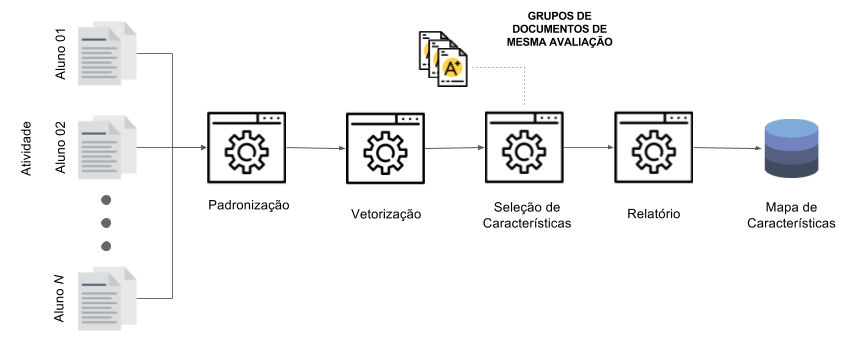
\includegraphics[width=.9\textwidth]{./img/mapa-alg-genetico.png}
\caption{Linha de execução do G.A. na otimização de cada classe de nota quanto ao número de características e a densidade dos agrupamentos.}
\label{mapa-alg-genetico}
\end{figure}

A representação apresentada na Figura \ref{mapa-alg-genetico} mostra o processo do texto com pré processamento, vetorização e a divisão em classes, individualmente entregues ao Algoritmo Genético objetivando a redução de dimensionalidade e seleção de características. Essas duas metas são necessárias para alcançar melhores resultados de classificação, pressupondo a existência de características chave para a resposta. Consideramos assim que existe uma resposta ótima possível que seja referência para a nota dada pelo professor. A estrutura do GA utilizado é apresentada na Figura \ref{calibracao-GA}.

\begin{figure}[th]
\centering
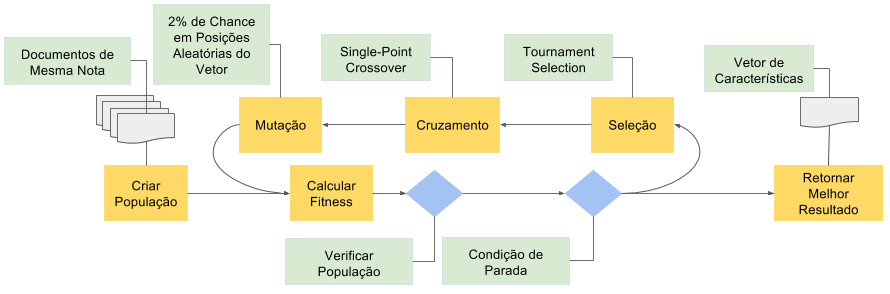
\includegraphics[width=.9\textwidth]{./img/estrutura-ga.png}
\caption{Estrutura do G.A. para seleção de características nas classes de nota.}
\label{calibracao-GA}
\end{figure}

Conforme representa a Figura \ref{calibracao-GA}, para início do GA o vetor dos documentos dos alunos é passado junto com o vetor de menor norma de cada grupo. Uma população aleatória é definida com vetores de tamanho \textit{k} características. A otimização inicia-se por esse menor que, em tese, deveria conter o requisito da avaliação tal como os outros itens do grupo de nota. Em cada geração do GA é executada a seleção \textit{por torneio}, aonde um par de cromossomos é selecionados aleatoriamente dentre a população e o de menor \textit{fitness} é retornado como um dos candidatos para \textit{cruzamento}. Após a definição de um par de vencedores é realizado o \textit{crossover}. Para isso, um índice randômico define o corte dos vetores, gerando dois novos vetores que correspondam à soma das partições desses primeiros. Esses vetores resultantes são submetidos à mutação. A chance de ocorrência é de 2\% e pode ocorrer em um número aleatório de genes do indivíduo, alternando o \textit{bit} dessas posições. Sem haver melhoria durante 700 gerações, o cromossomo de melhor \textit{fitness} é retornado como resultado.

No GA, para atribuir a cada indivíduo seu \textit{fitness} $f_{ind}$, primeiro calculamos a média de similaridade do agrupamento levando em conta as características selecionadas. Sendo o grupo \textit{S} formado por todos os documentos \textit{d} com mesma classificação na base de dados \textit{D}, é calculada a similaridade interna do agrupamento para os termos do indivíduo $ t_{ind} $. Então, o \textit{fitness}, dado pela Equação \ref{eq-fitness}, é o resultado da divisão do número de características selecionadas $ t_{ind} $ pela média de similaridade interna quando consideradas apenas as $ t_{ind} $ características.

\begin{equation}
Fitness_{f_{ind}} = \frac{t_{ind}}{\overline{x}_{sim_{s}}}
\label{eq-fitness}
\end{equation}

A métrica acima tende a selecionar características pela média de similaridade dos documentos, ou seja, através da densidade do grupo classificado pelo especialista. Assim, esperamos tornar os termos referenciados por essa classe mais próximos da avaliação. Assim, localizar quais características foram observadas pelos usuários é um desafio que deve ser aprofundado pois contém aspectos de classificação subjetiva ou interpretativa para atribuição de relevância por grupo de nota.


Segundo \citeonline{how2004}, algumas das formas de qualificar a seleção de características são: a análise de \textit{clusters}, métricas de distância, medidas estatísticas ou baseadas em teorias da informação. Um trabalho que realizou a comparação entre alguns métodos tradicionais de análise de relevância dos termos foi feito por \citeonline{algarni2014}. Nesse artigo os autores estudam o impacto na seleção de características de algumas técnicas de ponderação de relevância dos termos, semelhante à técnica de \textit{fitness} adotada, como \textit{Mutual Information}, \textit{Chi-Square}, \textit{Information Gain} e \textit{Odds Ratio}. 

Na Equação \ref{eq-fitness} foi utilizada portanto a medida de distância de similaridade interna para otimização da quantidade do conjunto de termos. A complexidade dessa seleção é dada pela atenção para um conjunto de termos objetivo (resposta) do usuário para além do modelo gerado pelo classificador. Os termos selecionados então, além do modelo avaliativo pretende representar uma descrição da atividade segundo o mapa de características. Experimentos que demonstram a aplicação dessa visão qualitativa das marcações segundo a resposta-base do professor são apresentados na Seção \ref{exp-mapas}.


Portanto, a calibração do GA foi observada com cautela. Existem bases de dados aos quais a apresentação de resultados de grande minimização têm muitos trechos visualmente equivalentes removidos. O contrário também ocorre, com pequenas minimizações e a marcação de grande porção de texto para a classe. Ambos os casos são importantes dependendo da atividade e do seu critério de avaliação.

Para contornar problemas de seleção textual, maximizado ou minimizado, foi implementada a inserção do documento de menor norma da classe como indivíduo inicial. Se o processo de avaliação for adequado ao critério, espera-se que esse elemento tenha o melhor \textit{fitness} dos documentos. Caso contrário, espera-se que os ciclos sejam capazes de contornar \textit{outliers} realizando testes com as demais características. Outra melhoria para acréscimo de liberdade de seleção ao GA foi o limite do número de gerações relativo a última melhoria. Essa alteração visava manter a influência de vetores selecionados para os próximos ciclos, mantendo a possibilidade de melhorias consecutivas.

Para definição dos parâmetros de população e número de gerações do GA, realizamos ciclos de testes com cinco processos paralelos. A população variou de 10 a 100 indivíduos em intervalos de 10 e o número de gerações de 100 a 1000 em intervalos de 100 com o objetivo de estudar a incidência do algoritmo genético nos extremos de densidade por classes. Para isso, foi escolhida a atividade \textit{TecII-5-8} com cinco classes sendo dois grupos desses de grande densidade e dois de pequena densidade. As notas maiores que representavam as classes '0' e '100' eram de otimização mais complexa pela menor densidade, ou seja, era maior a distância intra-cluster Equação \ref{eq-silhouette}. Enquanto as classes '90' e '93' eram respostas mais curtas e com maior densidade. Os resultados da otimização são listados na Tabela \ref{tab-ga-calibracao}.

 Observamos pela Tabela \ref{tab-ga-calibracao} os 15 melhores \textit{fitness} obtidos para cada classe. As de maior densidade apresentaram média de 700 gerações para retorno dos resultados. As de menor densidade por outro lado apresentaram resultados em média de 300 gerações. Para a população, foi comum a ocorrência das maiores independente do problema observado, tendo médias 90 e 100 em ambos. Assim, um número máximo foi definido como padrão, 100 de população e 700 gerações, para que o algoritmo tente atender, pelo menos, esses dois casos.

\begin{figure}
\centering
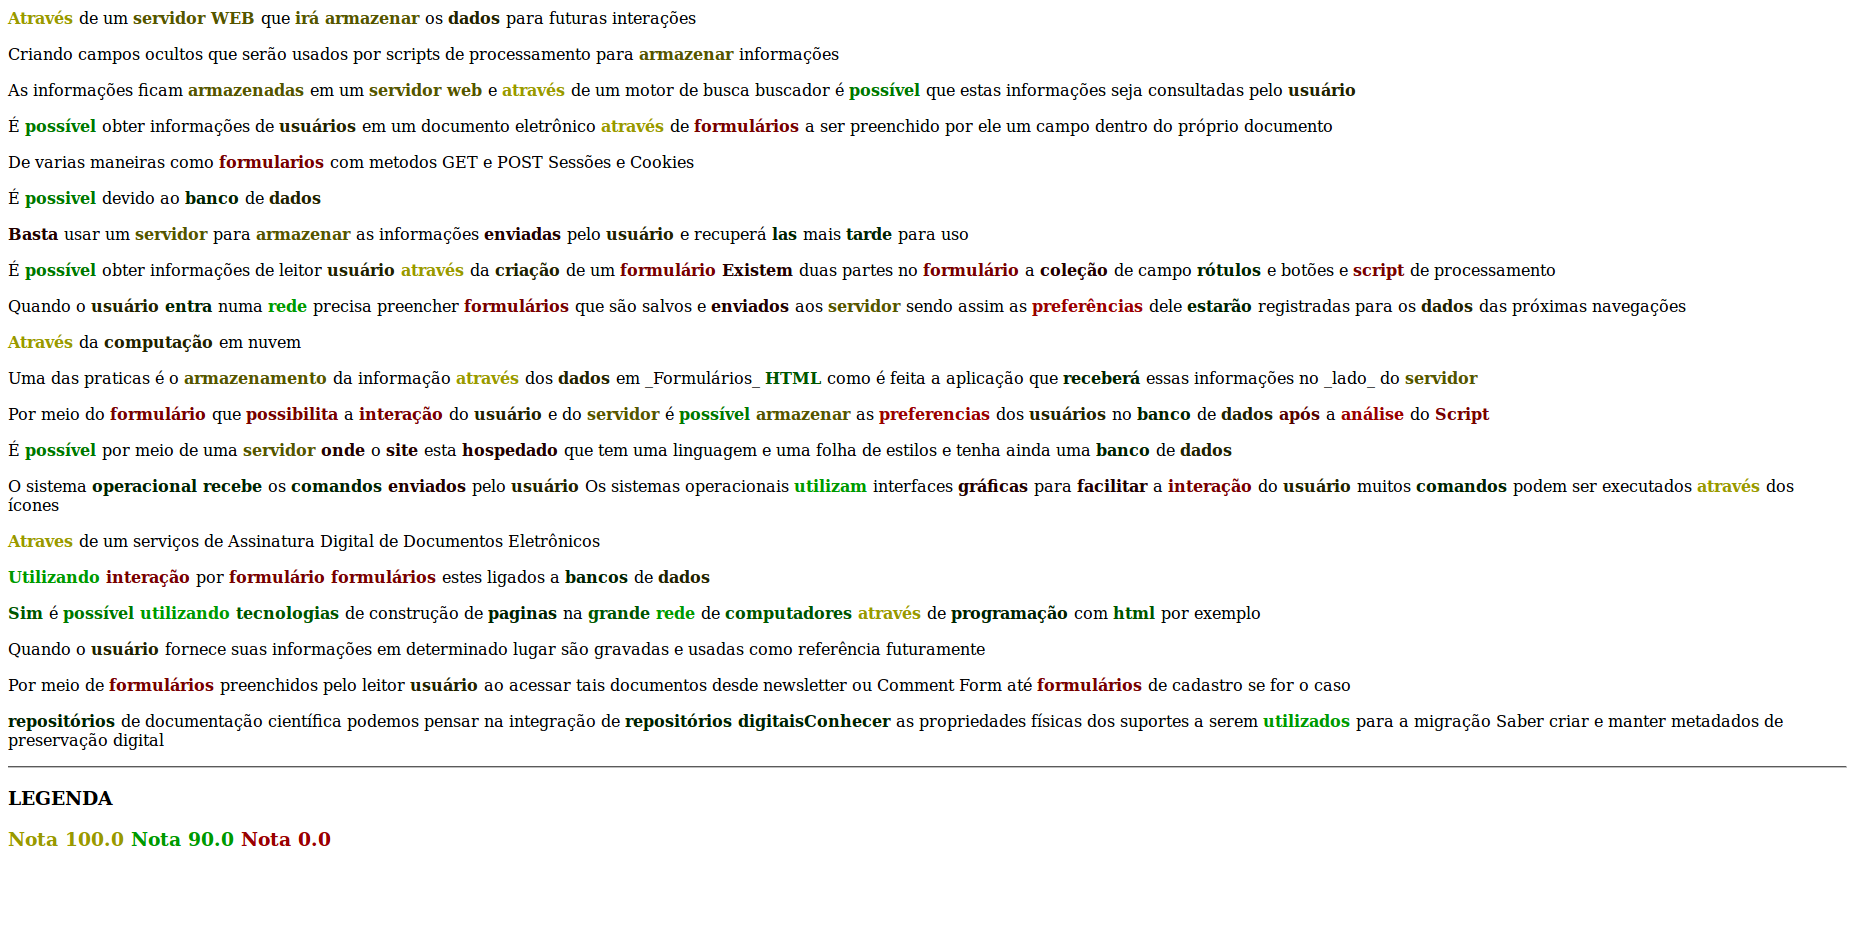
\includegraphics[angle=90, width=0.75\textwidth]{./img/Ufes186.png}
\caption{Visão geral do mapa de características como resultado da atividade Tec-II-5-186.}
\label{fig-ufes186}
\end{figure}

\section{{\it Feedbacks} e a Visualização das Características}

A etapa de identificação dos fatores relevantes elabora chaves de resposta que direcionam cada classe de nota ao respectivo conjunto de termos. Com a seleção do mapa de características através do GA, medindo cada ciclo de \textit{fitness}, o aumento da densidade das respostas torna o grupo mais conciso e melhora a identificação e a validação dos resultados. Porém, é importante salientar que os termos analisados de forma individualizada podem não caracterizar a resposta completa aguardada pelos professores por co-ocorrência de termos. Para isso, durante a produção desse sistema o pré processamento realizou seleções com faixas de 1 a 3-\textit{grams} para identificação de trechos compatíveis por classe.

Com os resultados em \textit{n-grams}, conseguimos identificar grandes trechos onde a grafia é semelhante. Com a seleção, os termos eliminados tornam os classificadores mais objetivos na avaliação por classe. Com isso, as características restantes resumem o grupo ao qual é associado de tal forma que os descreve. Assim, a seleção de características além de melhorar o desempenho dos sistemas de classificação é uma ferramenta de marcação e visualização dos resultados para visão sistêmica da questão e do conhecimento obtido.

Cada termo é associado ao grupo que ele descreve, gerando relatórios em HTML e em \LaTeX \cite{goossens1994}. Esses termos são marcados para todas as atividades, sendo treino ou teste dos algoritmos de avaliação. Em \LaTeX, o relatório é individual e apresenta ao professor criteriosamente sua avaliação. Em HTML é apresentando em uma escala de dez níveis para cada cor segundo uma nota, até no máximo seis notas. O nível é dado pela representatividade do termo na classe com as escalas RGB de 00 à 99. Um exemplo de marcação é dado na Figura \ref{fig-ufes186}  pela atividade 186 da disciplina de Tecnologia da Informação II da Universidade Federal do Espírito Santo.

Para a Figura \ref{fig-ufes186}, a atividade \textit{Tec-II-5-186} contém 4 classes distintas. As tonalidades das cores por nota, 100.0 em amarelo, 90.0 em verde e 0.0 em vermelho foram definidas conforme o peso dos fatores. Para cada palavra, o sistema apresentou o nível de representatividade do termo para a classe associada.

\begin{figure}[b]
\centering
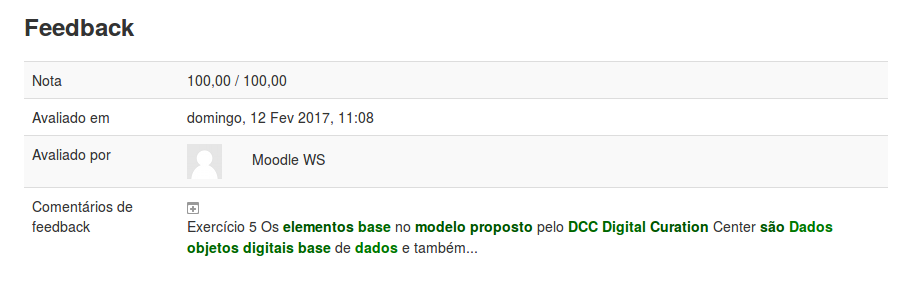
\includegraphics[width=\textwidth]{./img/mapa-ava.png}
\caption{Visualização do mapa de características como resultado individual no campo de \textit{feedback} do professor.}
\label{mapa-ava}
\end{figure}

O \textit{feedback} gerado pelo mapa de características é disponibilizado através do AVA no campo disponível para comentários do avaliador e o professor e os alunos podem utilizar as marcações para correções colaborativas. Com o reconhecimento das regiões, ambos têm os resultados como uma ferramenta para argumentar com o tema da questão e revisar o conteúdo pelo conhecimento dos participantes. Desse modo, além de melhoria dos processos internos de avaliação, o mapa formado durante o processo explica as soluções propostas para os participantes. Além disso, a ferramenta dá poder a todos os avaliados e avaliadores da discussão dos resultados. A resposta no Moodle, como nosso AVA padrão, pode ser vista na Figura \ref{mapa-ava}.

Os testes da classificação através da seleção de características e as comparações de resultados são apresentadas no Capítulo \ref{cap5}.